
%% bare_jrnl.tex
%% V1.0
%% 2016/05/20
%% by JIIST

%%
%% This is a skeleton file demonstrating the use of JIISTjrnl.cls
%% (requires JIISTjrnl.cls version 1.0 or later) with an JIIST journal paper.
%%
%% http://jiist.aiat.in.th/



% *** Authors should verify (and, if needed, correct) their LaTeX system  ***
% *** with the testflow diagnostic prior to trusting their LaTeX platform ***
% *** with production work. JIIST's font choices can trigger bugs that do  ***
% *** not appear when using other class files.                            ***
% The testflow support page is at:
% http://www.michaelshell.org/tex/testflow/


%%*************************************************************************
%% Legal Notice:
%% This code is offered as-is without any warranty either expressed or
%% implied; without even the implied warranty of MERCHANTABILITY or
%% FITNESS FOR A PARTICULAR PURPOSE! 
%% User assumes all risk.
%% In no event shall JIIST or any contributor to this code be liable for
%% any damages or losses, including, but not limited to, incidental,
%% consequential, or any other damages, resulting from the use or misuse
%% of any information contained here.
%%
%%
%% This work is distributed under the LaTeX Project Public License (LPPL)
%% ( http://www.latex-project.org/ ) version 1.3, and may be freely used,
%% distributed and modified. A copy of the LPPL, version 1.3, is included
%% in the base LaTeX documentation of all distributions of LaTeX released
%% 2003/12/01 or later.
%% Retain all contribution notices and credits.
%% ** Modified files should be clearly indicated as such, including  **
%% ** renaming them and changing author support contact information. **
%%
%%*************************************************************************

% Note that the a4paper option is mainly intended so that authors in
% countries using A4 can easily print to A4 and see how their papers will
% look in print - the typesetting of the document will not typically be
% affected with changes in paper size (but the bottom and side margins will).
% Use the testflow package mentioned above to verify correct handling of
% both paper sizes by the user's LaTeX system.
%
% Also note that the "draftcls" or "draftclsnofoot", not "draft", option
% should be used if it is desired that the figures are to be displayed in
% draft mode.
%
\documentclass[journal,transmag]{JIISTjrnl}
%
% If JIISTjrnl.cls has not been installed into the LaTeX system files,
% manually specify the path to it like:
% \documentclass[journal]{../sty/JIISTjrnl}





% Some very useful LaTeX packages include:
% (uncomment the ones you want to load)


% *** MISC UTILITY PACKAGES ***
%
%\usepackage{ifpdf}
% Heiko Oberdiek's ifpdf.sty is very useful if you need conditional
% compilation based on whether the output is pdf or dvi.
% usage:
% \ifpdf
%   % pdf code
% \else
%   % dvi code
% \fi
% The latest version of ifpdf.sty can be obtained from:
% http://www.ctan.org/tex-archive/macros/latex/contrib/oberdiek/
% Also, note that IEEEtran.cls V1.7 and later provides a builtin
% \ifCLASSINFOpdf conditional that works the same way.
% When switching from latex to pdflatex and vice-versa, the compiler may
% have to be run twice to clear warning/error messages.






% *** CITATION PACKAGES ***
%
%\usepackage{cite}
% cite.sty was written by Donald Arseneau
% V1.6 and later of JIISTjrnl pre-defines the format of the cite.sty package
% \cite{} output to follow that of JIIST. Loading the cite package will
% result in citation numbers being automatically sorted and properly
% "compressed/ranged". e.g., [1], [9], [2], [7], [5], [6] without using
% cite.sty will become [1], [2], [5]--[7], [9] using cite.sty. cite.sty's
% \cite will automatically add leading space, if needed. Use cite.sty's
% noadjust option (cite.sty V3.8 and later) if you want to turn this off.
% cite.sty is already installed on most LaTeX systems. Be sure and use
% version 4.0 (2003-05-27) and later if using hyperref.sty. cite.sty does
% not currently provide for hyperlinked citations.
% The latest version can be obtained at:
% http://www.ctan.org/tex-archive/macros/latex/contrib/cite/
% The documentation is contained in the cite.sty file itself.






% *** GRAPHICS RELATED PACKAGES ***
%
\ifCLASSINFOpdf
  % \usepackage[pdftex]{graphicx}
  % declare the path(s) where your graphic files are
  % \graphicspath{{../pdf/}{../jpeg/}}
  % and their extensions so you won't have to specify these with
  % every instance of \includegraphics
  % \DeclareGraphicsExtensions{.pdf,.jpeg,.png}
\else
  % or other class option (dvipsone, dvipdf, if not using dvips). graphicx
  % will default to the driver specified in the system graphics.cfg if no
  % driver is specified.
  % \usepackage[dvips]{graphicx}
  % declare the path(s) where your graphic files are
  % \graphicspath{{../eps/}}
  % and their extensions so you won't have to specify these with
  % every instance of \includegraphics
  % \DeclareGraphicsExtensions{.eps}
\fi
% graphicx was written by David Carlisle and Sebastian Rahtz. It is
% required if you want graphics, photos, etc. graphicx.sty is already
% installed on most LaTeX systems. The latest version and documentation can
% be obtained at: 
% http://www.ctan.org/tex-archive/macros/latex/required/graphics/
% Another good source of documentation is "Using Imported Graphics in
% LaTeX2e" by Keith Reckdahl which can be found as epslatex.ps or
% epslatex.pdf at: http://www.ctan.org/tex-archive/info/
%
% latex, and pdflatex in dvi mode, support graphics in encapsulated
% postscript (.eps) format. pdflatex in pdf mode supports graphics
% in .pdf, .jpeg, .png and .mps (metapost) formats. Users should ensure
% that all non-photo figures use a vector format (.eps, .pdf, .mps) and
% not a bitmapped formats (.jpeg, .png). JIIST frowns on bitmapped formats
% which can result in "jaggedy"/blurry rendering of lines and letters as
% well as large increases in file sizes.
%
% You can find documentation about the pdfTeX application at:
% http://www.tug.org/applications/pdftex





% *** MATH PACKAGES ***
%
%\usepackage[cmex10]{amsmath}
% A popular package from the American Mathematical Society that provides
% many useful and powerful commands for dealing with mathematics. If using
% it, be sure to load this package with the cmex10 option to ensure that
% only type 1 fonts will utilized at all point sizes. Without this option,
% it is possible that some math symbols, particularly those within
% footnotes, will be rendered in bitmap form which will result in a
% document that can not be JIIST Xplore compliant!
%
% Also, note that the amsmath package sets \interdisplaylinepenalty to 10000
% thus preventing page breaks from occurring within multiline equations. Use:
%\interdisplaylinepenalty=2500
% after loading amsmath to restore such page breaks as JIISTjrnl.cls normally
% does. amsmath.sty is already installed on most LaTeX systems. The latest
% version and documentation can be obtained at:
% http://www.ctan.org/tex-archive/macros/latex/required/amslatex/math/





% *** SPECIALIZED LIST PACKAGES ***
%
%\usepackage{algorithmic}
% algorithmic.sty was written by Peter Williams and Rogerio Brito.
% This package provides an algorithmic environment fo describing algorithms.
% You can use the algorithmic environment in-text or within a figure
% environment to provide for a floating algorithm. Do NOT use the algorithm
% floating environment provided by algorithm.sty (by the same authors) or
% algorithm2e.sty (by Christophe Fiorio) as JIIST does not use dedicated
% algorithm float types and packages that provide these will not provide
% correct JIIST style captions. The latest version and documentation of
% algorithmic.sty can be obtained at:
% http://www.ctan.org/tex-archive/macros/latex/contrib/algorithms/
% There is also a support site at:
% http://algorithms.berlios.de/index.html
% Also of interest may be the (relatively newer and more customizable)
% algorithmicx.sty package by Szasz Janos:
% http://www.ctan.org/tex-archive/macros/latex/contrib/algorithmicx/




% *** ALIGNMENT PACKAGES ***
%
%\usepackage{array}
% Frank Mittelbach's and David Carlisle's array.sty patches and improves
% the standard LaTeX2e array and tabular environments to provide better
% appearance and additional user controls. As the default LaTeX2e table
% generation code is lacking to the point of almost being broken with
% respect to the quality of the end results, all users are strongly
% advised to use an enhanced (at the very least that provided by array.sty)
% set of table tools. array.sty is already installed on most systems. The
% latest version and documentation can be obtained at:
% http://www.ctan.org/tex-archive/macros/latex/required/tools/


%\usepackage{mdwmath}
%\usepackage{mdwtab}
% Also highly recommended is Mark Wooding's extremely powerful MDW tools,
% especially mdwmath.sty and mdwtab.sty which are used to format equations
% and tables, respectively. The MDWtools set is already installed on most
% LaTeX systems. The lastest version and documentation is available at:
% http://www.ctan.org/tex-archive/macros/latex/contrib/mdwtools/


% JIISTjrnl contains the JIISTeqnarray family of commands that can be used to
% generate multiline equations as well as matrices, tables, etc., of high
% quality.


%\usepackage{eqparbox}
% Also of notable interest is Scott Pakin's eqparbox package for creating
% (automatically sized) equal width boxes - aka "natural width parboxes".
% Available at:
% http://www.ctan.org/tex-archive/macros/latex/contrib/eqparbox/





% *** SUBFIGURE PACKAGES ***
%\usepackage[tight,footnotesize]{subfigure}
% subfigure.sty was written by Steven Douglas Cochran. This package makes it
% easy to put subfigures in your figures. e.g., "Figure 1a and 1b". For JIIST
% work, it is a good idea to load it with the tight package option to reduce
% the amount of white space around the subfigures. subfigure.sty is already
% installed on most LaTeX systems. The latest version and documentation can
% be obtained at:
% http://www.ctan.org/tex-archive/obsolete/macros/latex/contrib/subfigure/
% subfigure.sty has been superceeded by subfig.sty.



%\usepackage[caption=false]{caption}
%\usepackage[font=footnotesize]{subfig}
% subfig.sty, also written by Steven Douglas Cochran, is the modern
% replacement for subfigure.sty. However, subfig.sty requires and
% automatically loads Axel Sommerfeldt's caption.sty which will override
% JIISTjrnl.cls handling of captions and this will result in nonJIIST style
% figure/table captions. To prevent this problem, be sure and preload
% caption.sty with its "caption=false" package option. This is will preserve
% JIISTjrnl.cls handing of captions. 
%
% The latest version and documentation can be obtained at:
% http://www.ctan.org/tex-archive/macros/latex/contrib/subfig/
% The latest version and documentation of caption.sty can be obtained at:
% http://www.ctan.org/tex-archive/macros/latex/contrib/caption/




% *** FLOAT PACKAGES ***
%
%\usepackage{fixltx2e}
% fixltx2e, the successor to the earlier fix2col.sty, was written by
% Frank Mittelbach and David Carlisle. This package corrects a few problems
% in the LaTeX2e kernel, the most notable of which is that in current
% LaTeX2e releases, the ordering of single and double column floats is not
% guaranteed to be preserved. Thus, an unpatched LaTeX2e can allow a
% single column figure to be placed prior to an earlier double column
% figure. The latest version and documentation can be found at:
% http://www.ctan.org/tex-archive/macros/latex/base/



%\usepackage{stfloats}
% stfloats.sty was written by Sigitas Tolusis. This package gives LaTeX2e
% the ability to do double column floats at the bottom of the page as well
% as the top. (e.g., "\begin{figure*}[!b]" is not normally possible in
% LaTeX2e). It also provides a command:
%\fnbelowfloat
% to enable the placement of footnotes below bottom floats (the standard
% LaTeX2e kernel puts them above bottom floats). This is an invasive package
% which rewrites many portions of the LaTeX2e float routines. It may not work
% with other packages that modify the LaTeX2e float routines. The latest
% version and documentation can be obtained at:
% http://www.ctan.org/tex-archive/macros/latex/contrib/sttools/
% Documentation is contained in the stfloats.sty comments as well as in the
% presfull.pdf file. Do not use the stfloats baselinefloat ability as JIIST
% does not allow \baselineskip to stretch. Authors submitting work to the
% JIIST should note that JIIST rarely uses double column equations and
% that authors should try to avoid such use. Do not be tempted to use the
% cuted.sty or midfloat.sty packages (also by Sigitas Tolusis) as JIIST does
% not format its papers in such ways.


%\ifCLASSOPTIONcaptionsoff
%  \usepackage[nomarkers]{endfloat}
% \let\MYoriglatexcaption\caption
% \renewcommand{\caption}[2][\relax]{\MYoriglatexcaption[#2]{#2}}
%\fi
% endfloat.sty was written by James Darrell McCauley and Jeff Goldberg.
% This package may be useful when used in conjunction with JIISTjrnl.cls'
% captionsoff option. Some JIIST journals/societies require that submissions
% have lists of figures/tables at the end of the paper and that
% figures/tables without any captions are placed on a page by themselves at
% the end of the document. If needed, the draftcls JIISTjrnl class option or
% \CLASSINPUTbaselinestretch interface can be used to increase the line
% spacing as well. Be sure and use the nomarkers option of endfloat to
% prevent endfloat from "marking" where the figures would have been placed
% in the text. The two hack lines of code above are a slight modification of
% that suggested by in the endfloat docs (section 8.3.1) to ensure that
% the full captions always appear in the list of figures/tables - even if
% the user used the short optional argument of \caption[]{}.
% JIIST papers do not typically make use of \caption[]'s optional argument,
% so this should not be an issue. A similar trick can be used to disable
% captions of packages such as subfig.sty that lack options to turn off
% the subcaptions:
% For subfig.sty:
% \let\MYorigsubfloat\subfloat
% \renewcommand{\subfloat}[2][\relax]{\MYorigsubfloat[]{#2}}
% For subfigure.sty:
% \let\MYorigsubfigure\subfigure
% \renewcommand{\subfigure}[2][\relax]{\MYorigsubfigure[]{#2}}
% However, the above trick will not work if both optional arguments of
% the \subfloat/subfig command are used. Furthermore, there needs to be a
% description of each subfigure *somewhere* and endfloat does not add
% subfigure captions to its list of figures. Thus, the best approach is to
% avoid the use of subfigure captions (many JIIST journals avoid them anyway)
% and instead reference/explain all the subfigures within the main caption.
% The latest version of endfloat.sty and its documentation can obtained at:
% http://www.ctan.org/tex-archive/macros/latex/contrib/endfloat/
%
% The JIISTjrnl \ifCLASSOPTIONcaptionsoff conditional can also be used
% later in the document, say, to conditionally put the References on a 
% page by themselves.





% *** PDF, URL AND HYPERLINK PACKAGES ***
%
%\usepackage{url}
% url.sty was written by Donald Arseneau. It provides better support for
% handling and breaking URLs. url.sty is already installed on most LaTeX
% systems. The latest version can be obtained at:
% http://www.ctan.org/tex-archive/macros/latex/contrib/misc/
% Read the url.sty source comments for usage information. Basically,
% \url{my_url_here}.





% *** Do not adjust lengths that control margins, column widths, etc. ***
% *** Do not use packages that alter fonts (such as pslatex).         ***
% (Unless specifically asked to do so by the journal or conference you plan
% to submit to, of course. )


% correct bad hyphenation here
\hyphenation{op-tical net-works semi-conduc-tor}
\usepackage{float}
\usepackage{fontspec}
\usepackage{graphicx}
\usepackage{algorithm}
%\usepackage{algorithmic}
%\usepackage{algpseudocode}
\usepackage{algcompatible}
\usepackage[table]{xcolor}
%\usepackage[table]{ycolor}
\usepackage{ragged2e,array,booktabs}
\usepackage[center]{caption}
%\usepackage{media9,graphicx}  %audio
\usepackage{graphicx}   %audio
% \usepackage[implicit=false]{hyperref}
%\usepackage{multimedia}
%\usepackage{attachfile}
%\usepackage{geometry}\geometry{verbose,letterpaper}\usepackage{movie15}\usepackage{hyperref}
%\usepackage[dvipdfmx]{movie15_dvipdfmx} \usepackage{hyperref}
\newcommand{\quotes}[1]{``#1''}
\newcommand{\enquote}[1]{``#1''}
\newfontfamily {\padauktext}[Script=Myanmar]{Padauk}
\newfontfamily\braillefont{SimBraille}
\DeclareTextFontCommand{\brailletext}{\braillefont}
\def\BibTeX{{\rm B\kern-.05em{\sc i\kern-.025em b}\kern-.08em
    T\kern-.1667em\lower.7ex\hbox{E}\kern-.125emX}}
\newenvironment{noeqnumber}
{\renewenvironment{equation}{\[}{\]}}{}
\begin{document}
%
% paper title
% can use linebreaks \\ within to get better formatting as desired
\title{Myanmar Text to Speech}
%
%
% author names and JIIST memberships
% note positions of commas and nonbreaking spaces ( ~ ) LaTeX will not break
% a structure at a ~ so this keeps an author's name from being broken across
% two lines.
% use \thanks{} to gain access to the first footnote area
% a separate \thanks must be used for each paragraph as LaTeX2e's \thanks
% was not built to handle multiple paragraphs


\author{Badounmar, Hnin Yu Hlaing, Hlaing May Tin, \\Nan Yu Hlaing, Thida San, Zun Hlaing Moe  
 
\thanks{Badounmar is with the Faculty of Computer Science, Computer University (Thaton), Thaton, Myanmar.}
\thanks{Hnin Yu Hlaing is with the Faculty of Information Science, University of Computer Studies(Meiktila), Meiktila, Myanmar.} 
\thanks{Hlaing May Tin is with the Faculty of Computer System and Technology, Myanmar Institute of Information Technology (MIIT), Mandalay, Myanmar.}      
\thanks{Nan Yu Hlaing, Zun Hlaing Moe and Thida San are with the Faculty of Information Science, Myanmar Institute of Information Technology (MIIT), Mandalay, Myanmar.}}

%\thanks{Zun Hlaing Moe, Thida San and Ei Thandar Phyu contributed equally to this work as first authors.}}
%\thanks{Manuscript received April 20, 2016; revised May 01, 2016.}}

% note the % following the last \JIISTmembership and also \thanks - 
% these prevent an unwanted space from occurring between the last author name
% and the end of the author line. i.e., if you had this:
% 
% \author{....lastname \thanks{...} \thanks{...} }
%                     ^------------^------------^----Do not want these spaces!
%
% a space would be appended to the last name and could cause every name on that
% line to be shifted left slightly. This is one of those "LaTeX things". For
% instance, "\textbf{A} \textbf{B}" will typeset as "A B" not "AB". To get
% "AB" then you have to do: "\textbf{A}\textbf{B}"
% \thanks is no different in this regard, so shield the last } of each \thanks
% that ends a line with a % and do not let a space in before the next \thanks.
% Spaces after \JIISTmembership other than the last one are OK (and needed) as
% you are supposed to have spaces between the names. For what it is worth,
% this is a minor point as most people would not even notice if the said evil
% space somehow managed to creep in.



% The paper headers
%\markboth{Journal of \LaTeX\ Class Files,~Vol.~6, No.~1, January~2016}%
%{Shell \MakeLowercase{\textit{et al.}}: Demo for JIIST Journals}
% The only time the second header will appear is for the odd numbered pages
% after the title page when using the twoside option.
% 
% *** Note that you probably will NOT want to include the author's ***
% *** name in the headers of peer review papers.                   ***
% You can use \ifCLASSOPTIONpeerreview for conditional compilation here if
% you desire.

% If you want to put a publisher's ID mark on the page you can do it like
% this:
%\JIISTpubid{0000--0000/00\$00.00~\copyright~2016 JIIST}
% Remember, if you use this you must call \JIISTpubidadjcol in the second
% column for its text to clear the JIISTpubid mark.



% use for special paper notices
%\JIISTspecialpapernotice{(Invited Paper)}





\JIISTtitleabstractindextext{%
\begin{abstract}
Text-to-speech system typically consists of a text analysis front-end, an acoustic model and a speech synthesizer. Since these components are trained independently and rely on extensive domain expertise. In this project to address these problems, we apply Tacotron2 through tensorflow, which is an end-to-end generated text-to-speech (TTS) model with syllable and word-level. Given <text, audio> pairs, the model can be trained from scratch with random initialization. End-to-end system can be trained on a small number of manually labeled text and audio paired data sets brings many advantages. In our experiment, according to the difficulties of the use of GPU, we trained 10 text and speech on step 10k for a week and investigated on closed test. Tacotron2 achieves a 3.8 subjective 5-scale mean opinion score on closed tests with listeners, outperforming a production parametric system in terms of naturalness. The clarity performance of the syllable-level is better than the word-level. In addition, since Tacotron2 generates speech at the frame level, it's substantially faster than sample-level autoregressive methods.
\end{abstract}
% JIISTjrnl.cls defaults to using nonbold math in the Abstract.
% This preserves the distinction between vectors and scalars. However,
% if the journal you are submitting to favors bold math in the abstract,
% then you can use LaTeX's standard command \boldmath at the very start
% of the abstract to achieve this. Many JIIST journals frown on math
% in the abstract anyway.

% Note that keywords are not normally used for peerreview papers.
\begin{JIISTkeywords}
TTS, Tacotron, Tensorflow, MOS, Encoder, Decoder
\end{JIISTkeywords}
}


% make the title area
\maketitle





% For peer review papers, you can put extra information on the cover
% page as needed:
% \ifCLASSOPTIONpeerreview
% \begin{center} \bfseries EDICS Category: 3-BBND \end{center}
% \fi
%
% For peerreview papers, this JIISTjrnl command inserts a page break and
% creates the second title. It will be ignored for other modes.
%\JIISTpeerreviewmaketitle



\section{Introduction}
% The very first letter is a 2 line initial drop letter followed
% by the rest of the first word in caps.
% 
% form to use if the first word consists of a single letter:
% \JIISTPARstart{A}{demo} file is ....
% 
% form to use if you need the single drop letter followed by
% normal text (unknown if ever used by JIIST):
% \JIISTPARstart{A}{}demo file is ....
% 
% Some journals put the first two words in caps:
% \JIISTPARstart{T}{his demo} file is ....
% 
% Here we have the typical use of a "T" for an initial drop letter
% and "HIS" in caps to complete the first word.
\JIISTPARstart{T}{he} main motivation for this project is to investigate the end-to-end text to speech synthesis with small corpus. TTS is a common research area of digital signal processing (DSP) and natural language processing (NLP). It is intended to generate human-like speech from the input text or sentences, a natural-sounding in terms of intelligibility and quality. The main task of TTS is to convert any text information into standard and smooth speech in real time. The speech synthesis is not a new problem, but it is still one of the challenges for organizations and businesses. The modern TTS trend is more complex.  Deep learning (DL) is a new research direction in the machine learning area in recent years. In this project, we experimented with TTS by Tacotron, one of deep learning methods which is to synthesize speech directly from the characters. It does not need phoneme-level alignment and can be trained on completely from scratch given <text, audio> pairs. There are a number of generative models already exist for this purpose, but some of them are not necessarily end-to-end as they usually have models developed and trained separately. Among these models, we used Tacotron as it is truly an end-to-end generative model that can fulfill our goal.\\
	The remainder of this paper is organized as follows. In Section 2, we describe the related work. Section 3 briefly introduces Myanmar Language. Section 4 describes methodology, Section 5 presents the overview of experimental setup, results and discussion. Lastly, we conclude in section 6.
% You must have at least 2 lines in the paragraph with the drop letter
% (should never be an issue)
%\hfill May 20, 2016
\section{Related Work} 
In recent years, DNN based generative models for Myanmar Speech synthesis can yield better synthesized speech than HMM \cite{b1}. In \cite{b2}, Quang Pham Huu proposed a deep learning architecture to the problem of speech synthesis, Tacotron model. The output of Tactron on both BigCorpus and SmallCorpus achieved high-quality speech audio. Lwin et al., proposed Tacotron-2 model synthesize speech directly from the characters and they experimented on Myanmar text and audio pairs \cite{b3}. Kim et al., researched a generative flow of speech synthesis with monotonic alignment search without any external aligner and they obtained the comparable speech quality to Tacotron-2 \cite{b4}. Chuxiong Zhang et al., introduced Tacotron for Mandrain Chinese TTS with prosodic features to generate more natural speech and obtained better by adding the prosodic system as the front-endsystem for Tacotron \cite{b6}. 
\section{Myanmar Language}
Myanmar language is the official language of Myanmar, and it is spoken as the first language by 32 million people and as the second language by another 10 million people. Myanmar script has 33 basic consonants, 4 basic medials, 12 basic vowels, other symbols and special characters. The consonants have only 23 distinct pronunciations because some consonants have the same pronunciation in the Myanmar language. A syllable is composed of one or more characters and one or more syllables can be formed as the word in Myanmar language. If the syllable final glottal stop is regarded as a tonal feature and the non-final neural vowel as anatonic vowel, there are four phonological tones in Myanmar \cite{b5}. 

\section{Methodology}
In this section, we describe the methodology used in this end-to-end text to speech synthesis. In the experiment of this project, used Tacotron2 was used with tensorflow.  
\subsection{Tacotron}
End-to-end speech synthesis system combines text analysis front-end, acoustic model and speech synthesizer into a unified framework without requiring phoneme level alignment and it can be trained on large scale of text and audio pairs with minimum human annotation. In this project, we used Tacotron-2, a fully end-to-end speech synthesis model that directly maps the input text to mel-spectrogram. The backbone of Tacotron is a seq2seq model with attention. Tacotron takes character sequence as inputs and outputs raw spectrograms which are later reconstructed using an algorithm called Griffin-Lim. It operates at frame-level which is why it is faster than sample-level auto-regressive models like WaveNet and SampleRNN. It consists of an encoder, an attention-based decoder, and a post-processing net. The encoder is responsible for building up a well-defined summarized representation of the input character sequence. The decoder has to learn about the alignment between the text representations and the output audio frames based on the context \cite{b3}. Figure ~\ref{Fig:1} depicts the model architecture, which includes an encoder, an attention-based decoder, and a post-processing network. On the high level, our model takes characters as input and the resulting spectral frame data is then converted to a waveform.
%\begin{equation}\label{eq:1}
%p(e,a|f)=\frac{\in}{(l_f+1)^{l_e}}\prod_{j=1}^{l_e}t(e_j|f_{a(j)})
%\end{equation}
\begin{figure}[H]
\centering
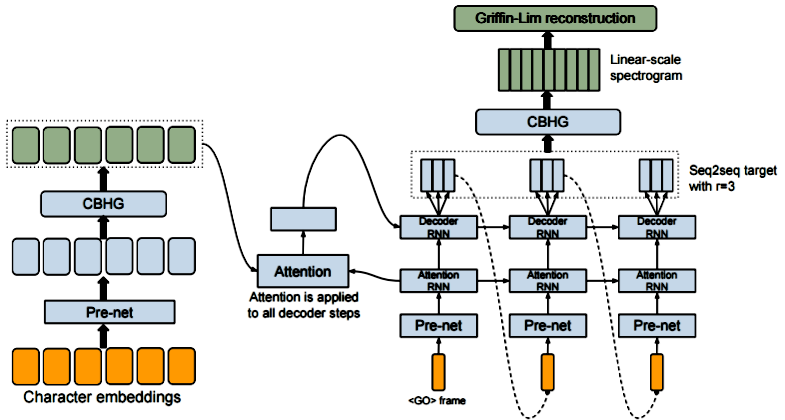
\includegraphics[width=3.5in]{tacotron.png}
% where an .eps filename suffix will be assumed under latex, 
% and a .pdf suffix will be assumed for pdflatex; or what has been declared
% via \DeclareGraphicsExtensions.
\caption{Model architecture. The model takes characters as input and outputs the corresponding raw spectrogram, which is then fed to the Graiffin-Lim reconstruction algorithm to synthesize speech}
\label{Fig:1}
\end{figure}
\subsection {CBHG Module}
CBHG consists of a one-dimensional convolution filter bank followed by a highway network and a two-way gated loop unit cyclic neural network (RNNCBHG is a powerful module to extract feature representations of sequences. A CNN works well for identifying simple patterns within your data which will then be used to form more complex patterns within higher layers. A 1D CNN is very effective when you expect to derive interesting features from shorter (fixed-length) segments of the overall data set and where the location of the feature within the segment is not of high relevance.
\subsection{Encoder}
The purpose of the encoder is to extract the robust sequence representation of the text. The input to the encoder is a sequence of characters, each character entered is a one-hot vector and embedded in a continuous vector. A set of non-linear transformations is then applied to each character vector, collectively referred to as "pre-net." The CBHG module transforms the output of the prenet into the final representation of the encoder and passes it to the subsequent attention module.
\subsection{Decoder}
Decoder turns the internal representation of the input signal into a Mel-spectrogram. A very important element of the network is the PostNet, designed to improve the spectrogram generated by the decoder.
\subsection{Post-Processing Network and Waveform Synthesis}
The post-processing network's task is to convert the output of seq2seq into a target representation that can be synthesized into a waveform. The CBHG module is used as a post-processing network. Waveform is synthesized from the predicted spectrogram using the Griffin-Lim algorithm. Griffin-Lim algorithm enables a partial restore of the signal after fast Fourier transforms. It can reduce artifacts, probably due to its harmonic enhancement. 
\section{Results and Discussion}
\subsection{Corpus Statistics}
For this experiment, we used sentences from the \quotes{Grade 2} Myanmar textbook published by the Ministry of Education. Firstly we prepared myanmar sentences and audio files. Myanmar sentences are segmented into syllable and word-level. For the syllable segmentation, we used a regular expression perl script developed by Saya Ye Kyaw Thu \cite{b7}.To prepare the speech corpus, we used audio that has been recorded for Myanmar Braille TTS. 
\subsection{Implementation}
To implement this project, we installed the following requirements:
\begin{itemize}
	\item 	Python3
	\item 	tensorflow framework  14.1 
	\item	numpy 1.19.2 
	\item	scikit-learn 0.20.3
	\item	librosa 3.0.3
	\item	falcon 1.2.0
	\item	tqdm  4.31.1
	\item	matploatlib 3.0.3
\end{itemize}
In the implementation, we prepared 10 sentences totally, this is for about 15 minutes in the format of text and audio parallel pair for training and two sentences for testing on closed test. Training time is a week for ten sentences. The maximum input text length is 117 and the maximum number of frames in the input audio is 6.
\subsection{Evaluation}
We used Mean Opinion Score (MOS) for the evaluation of the model output. Testing the outputs contains eleven listeners. We collected the evaluation rate from the listeners based on  three conditions: clarity, naturalness and accurate over 1-5 rating. Rating 5 is the best condition. Listeners answer the questions. For testing the clarity and naturalness they answer these questions \enquote{How could you hear the sound clarity? } and \enquote{ How does the sound is natural?}. For the accurate of the output sentence, we evaluate the condition based on this question \enquote{How many words can her the listener?} Calculate the accurate words based on how the listener hear the sentence accurately. For instance , there are six words in test sentence \enquote{{\padauktext ဘယ် ကို သွား ခဲ့ သ လဲ ။ }}. If the user hear only 4 words, we denote an accurate rate of 3.33 for that sentence . If the user hear all words, the accurate rate is 5. The MOS scores from the listeners are shown in figure ~\ref{Fig:6}. The genrerated output of syllable and word-level waveforms  are shown in figure ~\ref{Fig:2} to figure ~\ref{Fig:5}. According to figure ~\ref{Fig:5}, there is noise in the word-level generated waveform. Therefore, the intelligibility of syllable-level is better than the word-level. \\
\textbf{Input test sentence:}\hspace{7mm} {\padauktext အ ခန်း ( ၁ ) ။}\\
\textbf {Waveform for test sentence:}
\begin{figure}[H]
\centering
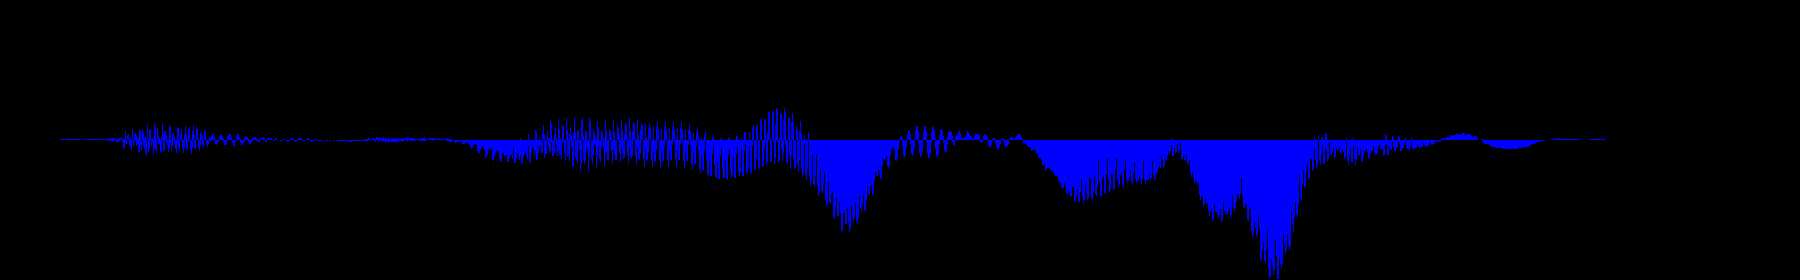
\includegraphics[width=2.5in]{Q1.png}
\caption{Syllable-Level Generated Waveform}
\label{Fig:2}
\end{figure}
\begin{figure}[H]
\centering
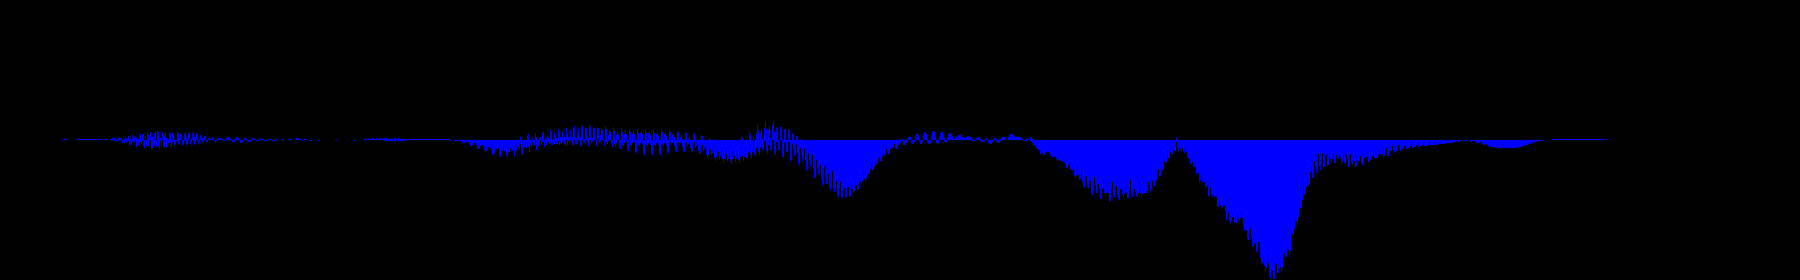
\includegraphics[width=2.5in]{wq1.png}
\caption{Word-Level Generated Waveform}
\label{Fig:3}
\end{figure}
\textbf{Input test sentence:}\hspace{7mm}{\padauktext ဘယ် ကို သွား ခဲ့ သ လဲ ။}\\
\textbf{Waveform for test sentence:}
\begin{figure}[H]
\centering
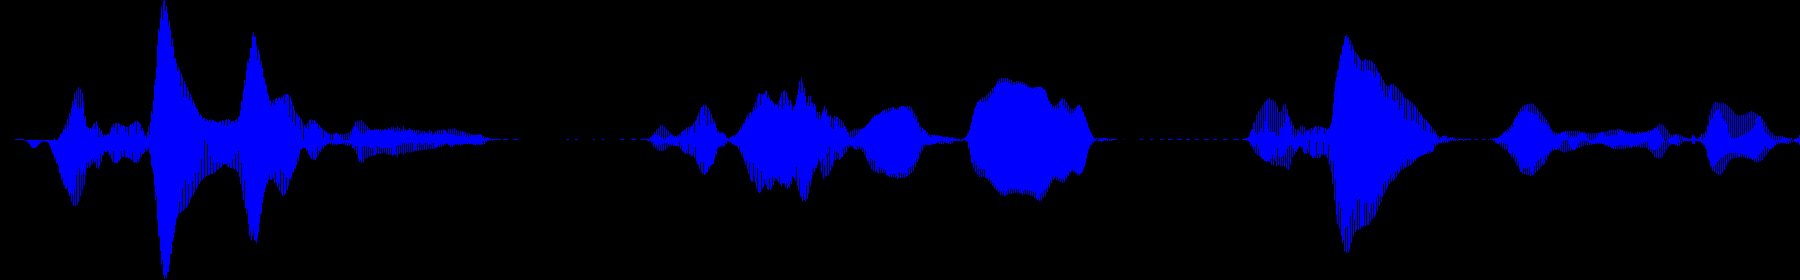
\includegraphics[width=2.5in]{Q2.png}
\caption{Syllable-Level Generated waveform}
\label{Fig:4}
\end{figure}
\begin{figure}[H]
\centering
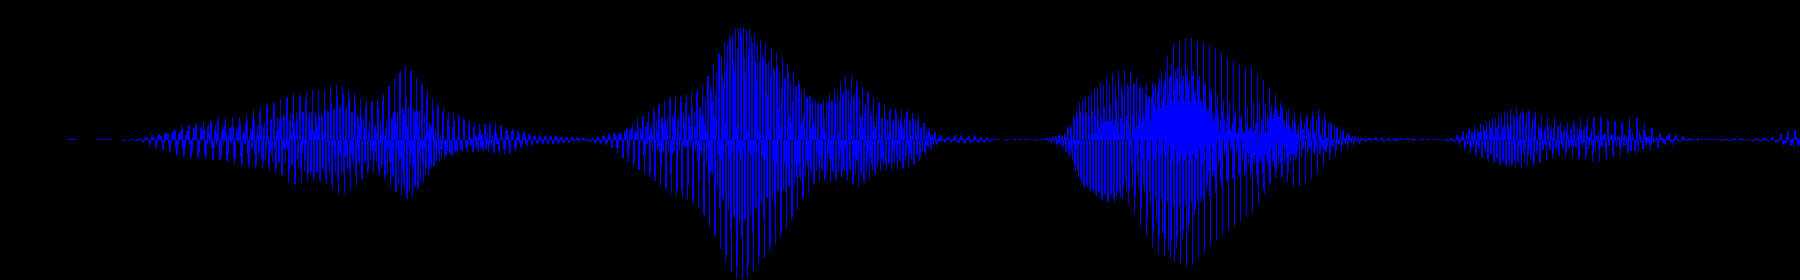
\includegraphics[width=2.5in]{wq2.png}
\caption{Word-Level Generated waveform}
\label{Fig:5}
\end{figure}
%%%%figure%%%%
%begin{figure}[ht]
%\includemovie[
%  poster,
%  text={\small(eval-58000-0.mp3)}
%]{6cm}{6cm}{Circle-m-increase3.mp4}
%\end{figure}
   % Created by James N{\"o}ckel, January 6, 2008:
  % \begin{figure}[h!]
  % \includemovie{550pt}{400pt}{eval-58000-0.mp3}
 %\end{figure}
  %\includemovie[3D]{height=3ex}{height=3ex>}{eval-58000-0.wav}

  %\movieref[play]{label spec}{Hi}
%Lezione 1: \includemedia[addresource=eval-58000-0.wav,transparent,flashvars={source=eval-58000-0.wav & autoPlay=true  },]          {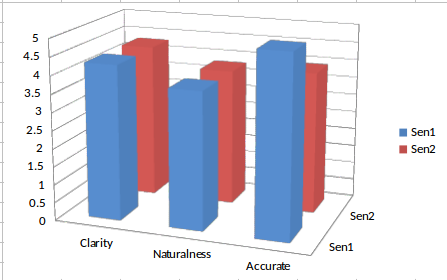
\includegraphics[height=3ex]{mos.png}{APlayer.swf}
%\sound[inlinesound]
%{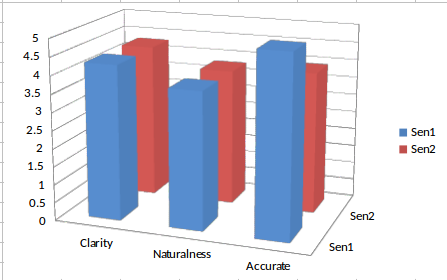
\includegraphics{mos.png}}{eval-58000-0.mp3}
%\includemovie[autoplay]{}{}{eval-58000-0.mp3}

According to figure ~\ref{Fig:7}:  clarity and naturalness of both test sentences are not significantly. However the first sentence is more accurate than the second one. According to our investigation, text length of the first sentence is shorter than the second and tonal significance is also better than the second one. Therefore the result of the first sentence is more better than the second one. The tone is also important for the text to speech.\\
\begin{figure}[H]
\centering
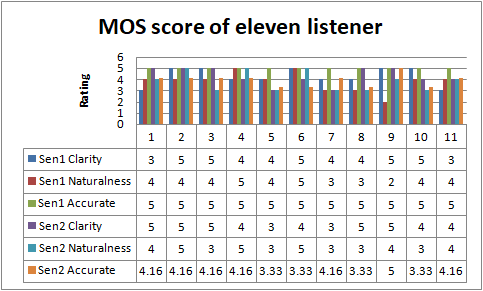
\includegraphics[width=3.5in]{score.png}
\caption{Rating Scores from the Listeners}
\label{Fig:6}
\end{figure}

\begin{figure}[H]
\centering
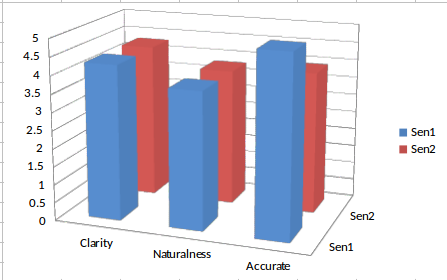
\includegraphics[width=3.5in]{mos.png}
\caption{Speech Quality of the Output Model}
\label{Fig:7}
\end{figure}

\section{Conclusion}
This mini project was contributed the evaluation of the end-to-end speech synthesis with tacorton model. This is the study of end-to-end speech synthesis with small corpus. We evaluated end-to-end TTS with the small corpus by using ten sentences  from \quotes{Grade 2} Myanmar Basic Education Textbook. Although the syllable-level achieved 3.8 MOS score, the word-level achieved 3.4 on closed tests with listeners. syllable-level also obtained more clearance result than word-level. Good speech output depends not only on recording condition but also on tone signature. By experimenting this mini project, we experienced that tacotron2 can work well even in a small corpus. In the near future, we will plan to test large corpus on tacotron2.


% if have a single appendix:
%\appendix[Proof of the Zonklar Equations]
% or
%\appendix  % for no appendix heading
% do not use \section anymore after \appendix, only \section*
% is possibly needed

% use appendices with more than one appendix
% then use \section to start each appendix
% you must declare a \section before using any
% \subsection or using \label (\appendices by itself
% starts a section numbered zero.)
%


%\appendices
%\section{Proof of the First Equation}
%Appendix one text goes here.

% you can choose not to have a title for an appendix
% if you want by leaving the argument blank
%\section{}
%Appendix two text goes here.


% use section* for acknowledgement

%The authors would like to thank...

% Can use something like this to put references on a page
% by themselves when using endfloat and the captionsoff option.
\ifCLASSOPTIONcaptionsoff
  \newpage
\fi



% trigger a \newpage just before the given reference
% number - used to balance the columns on the last page
% adjust value as needed - may need to be readjusted if
% the document is modified later
%\JIISTtriggeratref{8}
% The "triggered" command can be changed if desired:
%\JIISTtriggercmd{\enlargethispage{-5in}}

% references section

% can use a bibliography generated by BibTeX as a .bbl file
%\bibliographystyle{bibtex/JIISTjrnl}
% argument is your BibTeX string definitions and bibliography database(s)
%\bibliography{bibtex/JIIST,bibtex/example}
%
% <OR> manually copy in the resultant .bbl file
% set second argument of \begin to the number of references
% (used to reserve space for the reference number labels box)
\begin{thebibliography}{1}

%\bibitem{JIISThowto:kopka}
%H.~Kopka and P.~W. Daly, \emph{A Guide to \LaTeX}, 3rd~ed.\hskip 1em plus
 % 0.5em minus 0.4em\relax Harlow, England: Addison-Wesley, 1999.
\bibitem{b1} Aye Mya Hlaing, Win Pa Pa and Ye Kyaw Thu, \enquote{DNN based Myanmar Speech Synthesis}, The 6th Intl. Workshop on Spoken Language Technologies for Under-Resourced Languages 29-31 August 2018, pp, 142-146..
\bibitem{b2}  Quang Pham Huu, \enquote{The End-to-End Speech Synthesis System for the
VLSP Campaign 2019}.
\bibitem{b3} Htoo Pyae Lwin, Yuzana Win and Tomonari Masada, \enquote{Myanmar Text-to-Speech with End-to-End Speech Synthesis}.
\bibitem{b4} Jaehyeon Kim, Sungwon Kim, Jungil Kong and Sungroh Yoon, \enquote{ooo}, 34th Conference on Neural Information Processing Systems (NeurIPS 2020), Vancouver, Canada, pp, 1-11.
\bibitem{b5}U. Thein-Tun, \enquote{The domain of tones in burmese}, SST 1990 Proceedings, pp. 406--411, 1990.
\bibitem{b6}Chuxiong Zhang, Sheng Zhang and Haibing Zhong, \enquote{A Prosodic Mandarin Text-to-Speech System Basedon Tacotron}, Proceedings of APSIPA Annual Summit and Conference, 2019, pp, 165-169.
\bibitem{b7}https://github.com/ye-kyaw-thu/sylbreak.

\end{thebibliography}
% biography section
% % If you have an EPS/PDF photo (graphicx package needed) extra braces are
% needed around the contents of the optional argument to biography to prevent
% the LaTeX parser from getting confused when it sees the complicated
% \includegraphics command within an optional argument. (You could create
% your own custom macro containing the \includegraphics command to make things
% simpler here.)
%\begin{biography}[{\includegraphics[width=1in,height=1.25in,clip,keepaspectratio]{mshell}}]{Michael Shell}
% or if you just want to reserve a space for a photo:
%\begin{biography}[{\includegraphics[width=1in,height=1.25in,clip,keepaspectratio]{SYKT.pdf}}]{Ye Kyaw Thu}
%\begin{JIISTbiography}%{Ye Kyaw Thu}
% or if you just want to reserve a space for a photo:
%\parpic{\includegraphics[width=1in,clip,keepaspectratio]{headshot.jpg}}
%\section*{Group Members}
%\begin{itemize}
%	\item 	Badounmar\hspace{17mm}Ph.D(IT)-18
%	\item 	Hnin Yu Hlaing\hspace{10.7mm}Ph.D(IT)-10   
%	\item	Hlaing May Tin\hspace{10.3mm}Ph.D(IT)-6 
%	\item	Nan Yu Hlaing\hspace{12mm}Ph.D(IT)-16
%	\item	Thida San\hspace{19mm}Ph.D(IT)-12
%	\item	Zun Hlaing Moe\hspace{9.8mm}Ph.D(IT)-17
	
%\end{itemize}
%\vfill
%\attachfile[description={WWWWWWWWWWWWWWWWW}]{eval-58000-0.wav}
% Can be used to pull up biographies so that the bottom of the last one
% is flush with the other column.
%\enlargethispage{-5in}



% that's all folks
\end{document}


